
\documentclass[11pt]{article}
\PassOptionsToPackage{svgnames}{xcolor}
\usepackage{graphicx} % Required for inserting images
\usepackage[utf8]{inputenc}
\usepackage[margin=1in]{geometry}
\usepackage{enumerate, fancyhdr, color, verbatim, setspace, multirow, multicol,subcaption, booktabs, caption, amsfonts}
\usepackage{rotating}
\usepackage{amsmath}
\usepackage{amsthm}
\usepackage{listings}
\numberwithin{equation}{section}
\newtheorem{definition}{Definition}[subsection]
\newtheorem{theorem}{Theorem}[subsection]
\newtheorem{corollary}{Corollary}[subsection]

\usepackage{colortbl}
\usepackage{tikz}
\usetikzlibrary{matrix, positioning, shadings, shadows}
\usepackage{pgfplots}
\pgfplotsset{compat=1.18}
\usepackage[shortlabels]{enumitem}
% \usepackage[symbol]{footmisc}
\usepackage{multirow}
\usepackage{multicol}
% Creates the header and footer. You can adjust the look and feel of these here.
\usepackage{hyperref}
\hypersetup{
    colorlinks,
    citecolor=black,
    filecolor=black,
    linkcolor=blue,
    urlcolor=blue
}
\newcommand{\bp}{\mathbb{P}}

\definecolor{lightgray}{RGB}{230, 230, 230}
\definecolor{lightgrey}{RGB}{200, 200, 200}

\usepackage{tcolorbox}
\newenvironment{myblock}[1]{%
    \tcolorbox[beamer,%
    noparskip,breakable,
    colback=lightgray,colframe=black,%
    colbacklower=lightgrey,%
    title=#1]}%
    {\endtcolorbox}

\tcbuselibrary{skins,breakable}


\renewcommand{\headrulewidth}{0.2pt} %Creates a horizontal line underneath the header
\setlength{\headheight}{15pt} %Sets enough space for the header
% \renewcommand{\theenumi}{\alph{enumi}}
\onehalfspacing

\usepackage{chngcntr}
\counterwithin{figure}{section}

\DeclareMathOperator*{\argmin}{arg\,min}
\DeclareMathOperator*{\argmax}{arg\,max}

\usepackage[backend=biber, style=authoryear, maxcitenames=2, maxbibnames=9]{biblatex}
\DeclareDelimFormat{nameyeardelim}{\addcomma\space}
\addbibresource{references.bib}

\setcounter{tocdepth}{2}

\title{MGTECON 603 - Questions(Wk 2)\\ (Instructor: Guido Imbens)}
\author{Wooyong Park}
\date{\today}

\begin{document}


\maketitle

This is a document for the questions I had on the second week of the course.

\section{Slides 3 Neyman}

\subsection{Variance Calculation in the Population}

\begin{figure}[h]
    \centering
    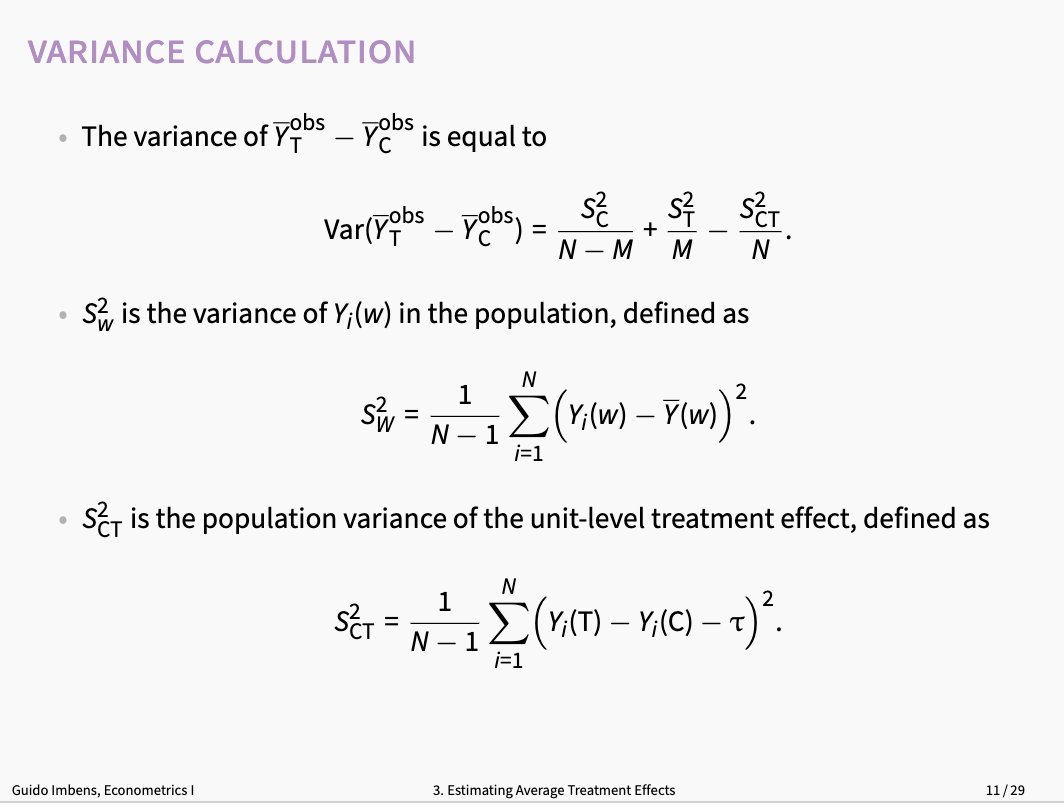
\includegraphics[width=0.7\textwidth]{images/wk2-2.png}
    \caption{Variance Calculation in the Population}
    \label{fig:variance-calculation}
\end{figure}

In the slide above, although the variance $S_W^2$ and $S_{CT}^2$ are defined in the population, the denominator is $N-1$ instead of $N$.
This is contradictory to what I learned in my undergraduate statistics course, where the population variance is defined as $\frac{1}{N} \sum_{i=1}^N (x_i - \mu)^2$.

Also, in this slide, I want to know how to derive the variance $V(\overline{Y}_T^{obs}-\overline{Y}_C^{obs}) = \frac{S_C^2}{N-M}+\frac{S_T^2}{M} - \frac{S_{CT}}{N}$; I have tried to derive it by myself, but I couldn't get the same result.


{
\color{blue}
Sarah's answer: The DoF correction in the denominator makes $S_W^2, S_{CT}^2$ unbiased estimators of the `super-population' variance.

}

\subsection{Covariates and the third term of the variance}

\begin{figure}[ht]
    \centering
    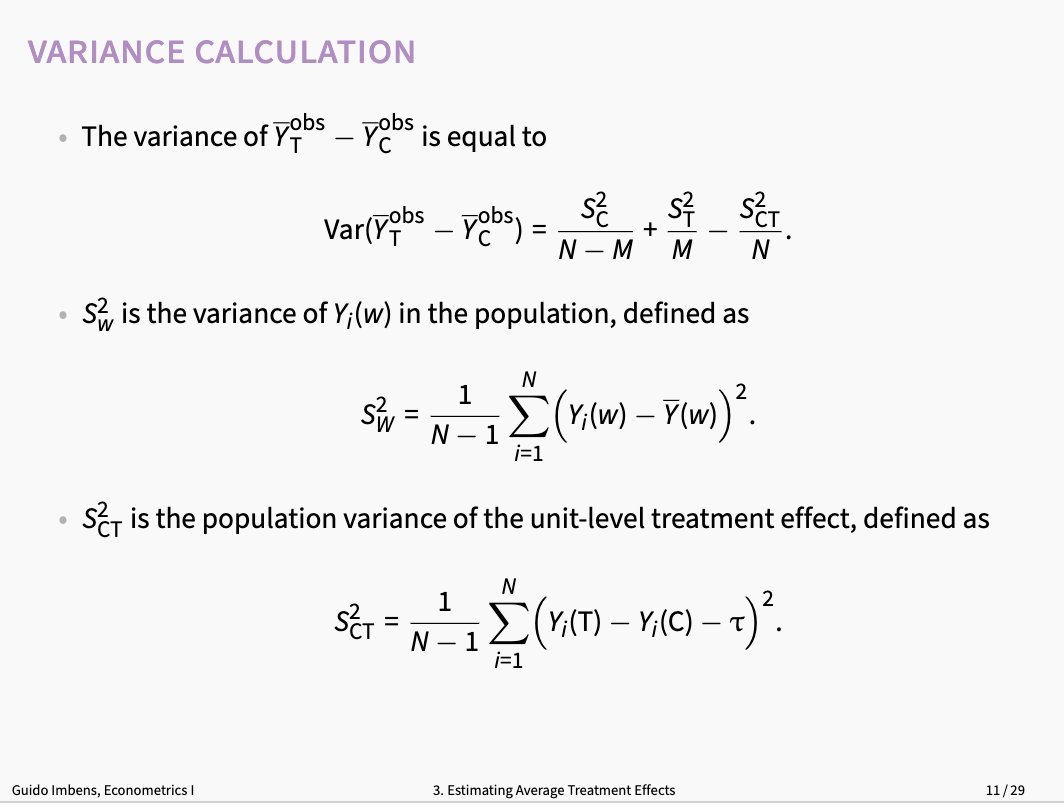
\includegraphics[width=0.7\textwidth]{images/wk2-2.png}
    \caption{Covariates and the third term of the variance}
    \label{fig:covariates-and-variance}
\end{figure}

In the slide above, the third term of the enitre variance of the difference-in-means, $S_{CT}^2$, is proportional to the heterogeneity of the treatment effects.
In Monday's lecture, the professor said that having covariates can increase precision by reducing this term.
However, I wonder if this is true for any kind of covariates. Giving this some thoughts, I think that if the covariates are colliders(i.e., $\{Y_i(0), Y_i(1)\} \perp W_i$ but $\{Y_i(0), Y_i(1)\} \perp W_i |X_i$),
this might bias the results from the beginning. 
Thus, I wonder if there are conditions that the covariates should satisfy to reduce the third term without biasing the estimation.

\section{Slides 4 OLS}

\subsection{Relationship between the linear model and the Potential Outcomes Framework}

In a private question with the professor, I asked about the relationship between the linear model and the Potential Outcomes Framework.
I wanted to know how the error term $\epsilon$ in the linear model is related to the potential outcomes $Y_i(0)$ and $Y_i(1)$.
In most cases, I find that the unconfoundedness assumption, $\{Y_i(0), Y_i(1)\} \perp W_i | X_i$, corresponds to the assumption that the error term $\epsilon$ is uncorrelated with the treatment $W_i$ when $X_i$ is included in the model.

The professor answered that the error term can be interpreted as $\varepsilon_i = Y_i(0) - X_i'\beta$, where $X_i'$ is the vector of covariates excluding the treatment indicator.
In a simple linear regression without covariates, it would be $\varepsilon_i = Y_i(0) - \alpha$.
In this case, regarding $Y_i(0)$ as constants or predetermined does not make sense, as $\varepsilon_i$ is a random variable.
Then, would the Neyman interpretation of the $Y_i(0)$ as constants or predetermined still hold?


{\color{blue}
Sarah's answer and a little bit of my interpretation: The super-population interpretation of randomized experiments, which follows from OLS, assumes that the stochasticity comes from resampling from a super-population, not from the permutation of the treatment.
Thus, $Y_i(0)$ is a random variable sampled from a super-population, and $\varepsilon_i$ inherits that randomness.

}

\end{document}
